\documentclass[10pt]{article}

% ---------- IDIOMA Y CODIFICACIÓN ----------
\usepackage[utf8]{inputenc}
\usepackage[spanish]{babel}
\usepackage{amsmath}
\usepackage[margin=2.5cm]{geometry}
\usepackage{setspace}
\usepackage{graphicx}
\usepackage{listings}
\usepackage{tikz}
\usetikzlibrary{circuits.logic.US}

% ---------- TABLAS (Actividad 1: identificación de dispositivos) ----------
\usepackage{booktabs}   % líneas de tabla profesionales (\toprule, \midrule, \bottomrule)
\usepackage{array}
\usepackage{ragged2e}
\usepackage[table]{xcolor} % opcional, para color en encabezado
\usepackage{tabularx}   % columnas que se ajustan al ancho de página
\usepackage{longtable}  % tablas que pueden partirse entre páginas (útil si tu tabla de dispositivos es larga)
\usepackage{caption}    % control de estilo de "Tabla X: ..."
\usepackage{float}
\usepackage{makecell}

% ---------- GLOSARIO (Actividad 2) ----------
% Enfoque simple con "description", sin necesidad de correr makeglossaries aparte
% (evita agregar un paso extra a tu pipeline de compilación).
\usepackage{enumitem}
\newlist{glosario}{description}{1}
\setlist[glosario]{
    font=\normalfont\bfseries,
    leftmargin=0pt,
    labelsep=0.5em,
    itemsep=0.5em
}

% ------- TABLAS PARA EMULADOR 8086 ---
% Uso dentro del documento:
%   \begin{glosario}
%       \item[Chipset] Definición y características...
%   \end{glosario}

% ---------- PLACEHOLDER \relleno ----------
% Uso: \relleno              -> texto de aviso genérico
%      \relleno{Tu texto}    -> muestra tu texto en rojo (útil para ir dejando borradores)
\newcommand{\relleno}[1][\textbf{[COMPLETAR AQUÍ]}]{\textcolor{red}{#1}}
% ---------- CONFIGURACIONES PARA ENCABEZADO Y PORTADA ----------
\usepackage{colortbl}
\usepackage[colorlinks=true,linkcolor=black,urlcolor=black,citecolor=black]{hyperref}

% Definición de colores y columnas personalizadas (usadas en la portada)
\definecolor{tablebackground}{rgb}{0.8, 0, 0}
\newcolumntype{x}[1]{>{\centering\arraybackslash\hspace{0pt}}p{#1}}
\newcolumntype{M}[1]{>{\centering\arraybackslash}m{#1}}
\newcolumntype{N}{@{}m{0pt}@{}}
\newcolumntype{P}[1]{>{\RaggedRight\arraybackslash}p{#1}}

% Variables de datos para la portada y encabezado
\newcommand{\itemEmail}{ccapatinta@unsa.edu.pe}
\newcommand{\itemStudent}{Camilo B.A. Capatinta Almanza (Teoría grupo B)}
\newcommand{\itemCourse}{Lab. Arq. de computadoras}
\newcommand{\itemCourseCode}{1702227}
\newcommand{\itemSemester}{IV}
\newcommand{\itemUniversity}{Universidad Nacional de San Agustín de Arequipa}
\newcommand{\itemFaculty}{Facultad de Ingeniería de Producción y Servicios}
\newcommand{\itemDepartment}{Departamento Académico de Ingeniería de Sistemas e Informática}
\newcommand{\itemSchool}{Escuela Profesional de Ingeniería de Sistemas}
\newcommand{\itemAcademic}{2026 - B}
\newcommand{\itemInput}{13/10/2026}
\newcommand{\itemOutput}{--/10/2026}
\newcommand{\itemPracticeNumber}{04}
\newcommand{\itemTheme}{Programación para el microprocesador INTEL - Instrucciones Lógicas y Registro de Banderas}

% Configuración del encabezado y pie de página (fancyhdr)
\usepackage{fancyhdr}
\pagestyle{fancy}
\fancyhf{}
\setlength{\headheight}{40.51407pt}
\renewcommand{\headrulewidth}{1pt}
\renewcommand{\footrulewidth}{1pt}

% Encabezado
\fancyhead[L]{\raisebox{-0.2\height}{
\includegraphics[width=3cm]{img/logo_episunsa.png}}}
\fancyhead[C]{\fontsize{7}{7}\selectfont    \itemUniversity \\ \itemFaculty \\ \itemDepartment \\ \itemSchool \\ \textbf{\itemCourse}}
\fancyhead[R]{\raisebox{-0.2\height}{
\includegraphics[width=1.2cm]{img/logo_abet.png}}}

% Pie de página
\fancyfoot[L]{Estudiante Camilo Capatinta}
\fancyfoot[C]{\itemCourse}
\fancyfoot[R]{Página \thepage}

\begin{document}

% --- INICIO DE LA PORTADA ---
	\vspace*{10px}
	
	\begin{center}
		\parbox{0.8\textwidth}{\centering\fontsize{17}{20}\selectfont\textbf{Informe de laboratorio \itemPracticeNumber}}
	\end{center}
	\begin{center}
		\parbox{0.8\textwidth}{\centering\textbf{\Large Tema: \itemTheme}}
	\end{center}

\begin{flushright}
    \begin{tabular}{|M{2.5cm}|N|}
        \hline 
        \rowcolor{tablebackground}
        \color{white} \textbf{Nota}  \\
        \hline 
             \\[30pt]
        \hline          
    \end{tabular}
\end{flushright}    

\begin{table}[h!]
    \begin{tabular}{|x{4.7cm}|x{4.8cm}|x{4.8cm}|}        
        \hline 
        \rowcolor{tablebackground}
        \color{white} \textbf{Estudiante} & \color{white}\textbf{Escuela}  & \color{white}\textbf{Asignatura}   \\
        \hline 
        {\itemStudent \par \itemEmail} & \itemSchool & {\itemCourse \par Semestre: \itemSemester \par Código: \itemCourseCode}     \\
        \hline          
    \end{tabular}
\end{table}     

\begin{table}[H]
    \begin{tabular}{|x{4.7cm}|x{4.8cm}|x{4.8cm}|}
        \hline 
        \rowcolor{tablebackground}
        \color{white}\textbf{Laboratorio} & \color{white}\textbf{Tema}  & \color{white}\textbf{Duración}   \\
        \hline 
        \itemPracticeNumber & \itemTheme & 02 horas   \\
        \hline 
    \end{tabular}
\end{table}

\begin{table}[H]
    \begin{tabular}{|x{4.7cm}|x{4.8cm}|x{4.8cm}|}
        \hline 
        \rowcolor{tablebackground}
        \color{white}\textbf{Semestre académico} & \color{white}\textbf{Fecha de inicio}  & \color{white}\textbf{Fecha de entrega}   \\
        \hline 
        \itemAcademic & \itemInput &  \itemOutput  \\
        \hline 
    \end{tabular}
\end{table}

\newpage
\tableofcontents
\thispagestyle{plain}
\clearpage

% ---------- Definiciones auxiliares ----------
\lstdefinestyle{asm}{
  language={[x86masm]Assembler},
  basicstyle=\ttfamily\small,
  keywordstyle=\bfseries,
  commentstyle=\itshape,
  numbers=left,
  numberstyle=\tiny,
  numbersep=6pt,
  frame=single,
  breaklines=true,
  showstringspaces=false,
  tabsize=4
}
 
\newcommand{\espacioimagen}[1]{%
  \fbox{\parbox[c][4.5cm][c]{0.9\linewidth}{\centering\itshape Insertar captura: #1}}}
 
% \figuraimagen{archivo.png}{Leyenda}{etiqueta}{descripción del recuadro}
\newcommand{\figuraimagen}[4]{%
  \begin{figure}[htbp]
    \centering
    \IfFileExists{img/#1}{\includegraphics[width=0.9\linewidth]{img/#1}}{\espacioimagen{#4}}
    \caption{#2}\label{#3}
  \end{figure}}
 


\section{Objetivos}
 
\textbf{Objetivo general.} Analizar la forma en que se ejecutan algunas instrucciones lógicas observando cómo estas afectan al registro de estados.

\textbf{Objetivos específicos.}
\begin{itemize}
  \item Examinar detenidamente la manera en que se ejecutan algunas instrucciones lógicas.
  \item Analizar la manera en que se modifica el registro de banderas, dependiendo del tipo de operación y los datos que operan.
  \item Identificar las características propias de las máscaras que se utilizan junto con las instrucciones lógicas.
\end{itemize}
 
% ============================================================
\section{Materiales y equipos}
 
\begin{itemize}
  \item Guía de laboratorio.
  \item Computadora PC con el programa EMU8086.
\end{itemize}
 
% ============================================================
\section{Actividades}
 
\subsection{Preparación del entorno}
 
\begin{itemize}
  \item Se ejecutó el emulador EMU8086 y se creó un nuevo documento tipo COM.
  \item Cada programa se escribió con su encabezado \texttt{\#make\_COM\#} y \texttt{org 100h}, necesario para generar un archivo \texttt{.COM}.
  \item Para observar las banderas se usó el botón \textbf{flags} de la ventana del emulador junto con la ejecución paso a paso (\textit{single step}).
\end{itemize}
 
Las banderas que se monitorearon se resumen en la Tabla~\ref{tab:banderas}.
 
\begin{table}[htbp]
  \centering
  \caption{Banderas del registro de estados utilizadas en la práctica.}
  \label{tab:banderas}
  \begin{tabular}{|c|p{3cm}|p{5.5cm}|}
    \hline
    \textbf{Bandera} & \textbf{Nombre} & \textbf{Se activa (=1) cuando\ldots} \\
    \hline
    Z & Cero & el resultado de la operación es 0. \\
    \hline
    S & Signo & el bit más significativo del resultado es 1 (bit 7 en operaciones de 8 bits, bit 15 en las de 16 bits). \\
    \hline
    P & Paridad & el byte bajo del resultado tiene un número par de unos. \\
    \hline
    C, O & Acarreo y desbordamiento & \texttt{AND}, \texttt{OR} y \texttt{XOR} las dejan siempre en 0. \\
    \hline
    D, I & Dirección e interrupción & se modifican con instrucciones específicas (\texttt{STD/CLD}, \texttt{STI/CLI}). \\
    \hline
  \end{tabular}
\end{table}
 
% ------------------------------------------------------------
\subsection{Primer programa: AND, OR y XOR con máscaras}
 
\textbf{Objetivo.} Observar cómo las instrucciones \texttt{AND}, \texttt{OR} y \texttt{XOR} operan sobre registros de 8 y 16 bits usando máscaras, y cómo cada una actualiza las banderas. El programa declara sus datos con las directivas \texttt{DB} y \texttt{DW}.
 
\textbf{Funcionamiento.}
\begin{itemize}
  \item \texttt{DL = dato1 AND mascara1} (8 bits).
  \item \texttt{CX = dato2 AND mascara2} (16 bits).
  \item \texttt{CX = CX AND CX}: no cambia CX, solo actualiza las banderas.
\end{itemize}
 
\begin{figure}[H]
    \centering
    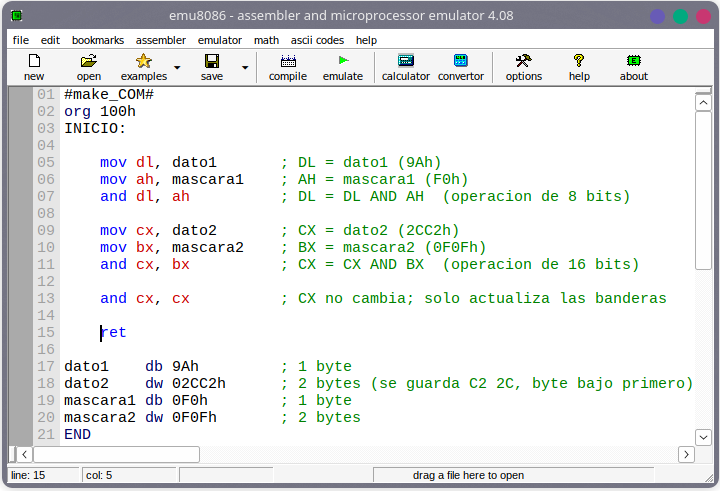
\includegraphics[width=0.8\textwidth]{img/1.png}
    \caption{Código del primer programa en el editor de EMU8086.}
    \label{fig:programa1.com}
\end{figure}

\textbf{Procedimiento.}
\begin{itemize}
  \item Se compiló y se ejecutó paso a paso, anotando tras cada \texttt{AND} los operandos, el resultado y las banderas (Tabla~\ref{tab:p1-and}).
  \item Se sustituyeron las tres instrucciones \texttt{AND} por \texttt{OR} y se repitió el procedimiento (Tabla~\ref{tab:p1-or}).
  \item Se sustituyeron por \texttt{XOR} y se repitió nuevamente (Tabla~\ref{tab:p1-xor}).
\end{itemize}
 
\begin{table}[htbp]
  \centering
  \caption{Resultados del primer programa con \texttt{AND}.}
  \label{tab:p1-and}
  \begin{tabular}{|l|c|c|c|c|c|c|}
    \hline
    \textbf{Instrucción} & \textbf{Operandos} & \textbf{Resultado} & \textbf{S} & \textbf{Z} & \textbf{P} & \textbf{C/O} \\
    \hline
    \texttt{and dl, ah} & 9Ah, F0h & 90h & 1 & 0 & 1 & 0/0 \\
    \hline
    \texttt{and cx, bx} & 2CC2h, 0F0Fh & 0C02h & 0 & 0 & 0 & 0/0 \\
    \hline
    \texttt{and cx, cx} & 0C02h, 0C02h & 0C02h & 0 & 0 & 0 & 0/0 \\
    \hline
  \end{tabular}
\end{table}

\begin{figure}[H]
    \centering
    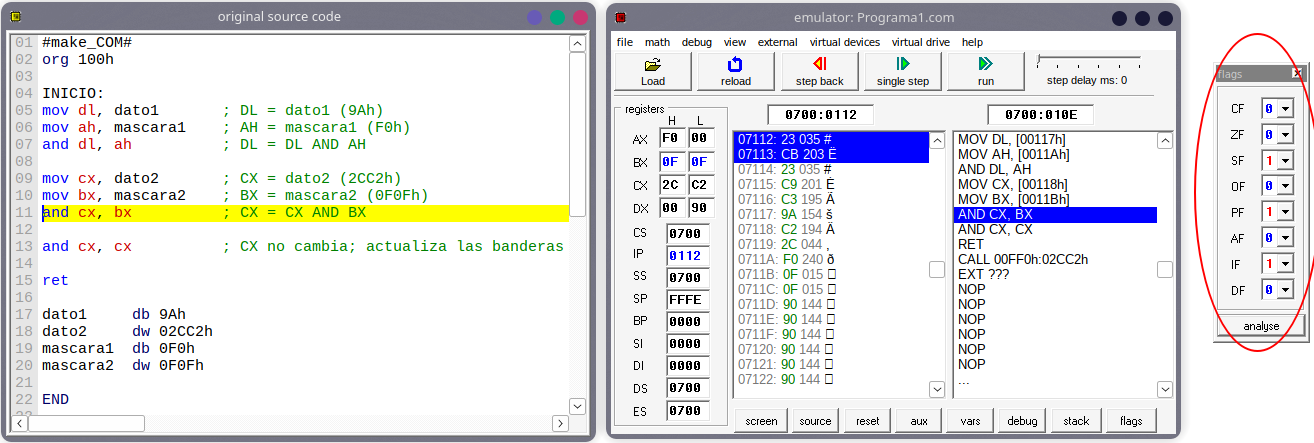
\includegraphics[width=0.91\textwidth]{img/2.png}
    \caption{Registros y banderas ejecutando las instrucciones AND.}
    \label{fig:programa1.com}
\end{figure}
  
\begin{table}[htbp]
  \centering
  \caption{Resultados del primer programa con \texttt{OR}.}
  \label{tab:p1-or}
  \begin{tabular}{|l|c|c|c|c|c|c|}
    \hline
    \textbf{Instrucción} & \textbf{Operandos} & \textbf{Resultado} & \textbf{S} & \textbf{Z} & \textbf{P} & \textbf{C/O} \\
    \hline
    \texttt{or dl, ah} & 9Ah, F0h & FAh & 1 & 0 & 1 & 0/0 \\
    \hline
    \texttt{or cx, bx} & 2CC2h, 0F0Fh & 2FCFh & 0 & 0 & 1 & 0/0 \\
    \hline
    \texttt{or cx, cx} & 2FCFh, 2FCFh & 2FCFh & 0 & 0 & 1 & 0/0 \\
    \hline
  \end{tabular}
\end{table}
 
\begin{figure}[H]
    \centering
    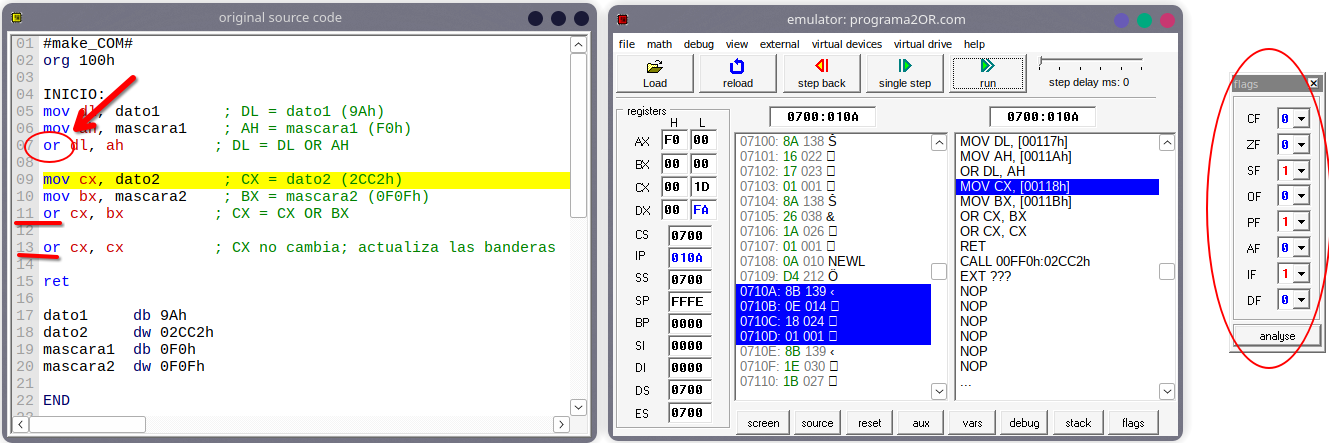
\includegraphics[width=0.91\textwidth]{img/3.png}
    \caption{Registros y banderas ejecutando las instrucciones OR.}
    \label{fig:programa1OR.com}
\end{figure}

\begin{table}[htbp]
  \centering
  \caption{Resultados del primer programa con \texttt{XOR}.}
  \label{tab:p1-xor}
  \begin{tabular}{|l|c|c|c|c|c|c|}
    \hline
    \textbf{Instrucción} & \textbf{Operandos} & \textbf{Resultado} & \textbf{S} & \textbf{Z} & \textbf{P} & \textbf{C/O} \\
    \hline
    \texttt{xor dl, ah} & 9Ah, F0h & 6Ah & 0 & 0 & 1 & 0/0 \\
    \hline
    \texttt{xor cx, bx} & 2CC2h, 0F0Fh & 23CDh & 0 & 0 & 0 & 0/0 \\
    \hline
    \texttt{xor cx, cx} & 23CDh, 23CDh & 0000h & 0 & 1 & 1 & 0/0 \\
    \hline
  \end{tabular}
\end{table}
 
\begin{figure}[H]
    \centering
    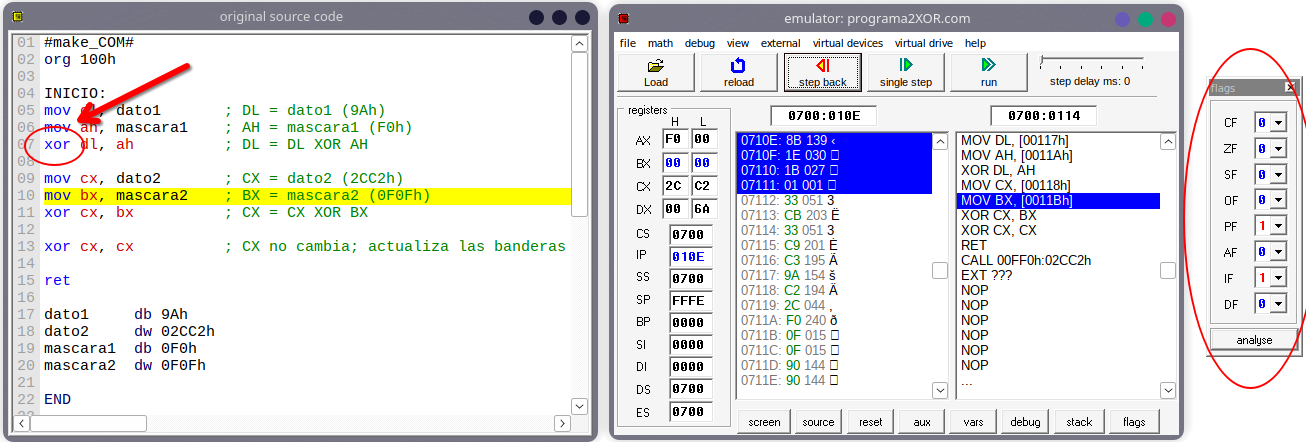
\includegraphics[width=0.91\textwidth]{img/4.png}
    \caption{Registros y banderas ejecutando las instrucciones OR.}
    \label{fig:programa1XOR.com}
\end{figure}
 
\textbf{Observaciones.} Con la máscara F0h, \texttt{AND} conserva el nibble alto y borra el bajo (90h), \texttt{OR} pone en 1 el nibble alto y conserva el bajo (FAh) y \texttt{XOR} invierte el nibble alto y conserva el bajo (6Ah). En las tres operaciones C y O quedaron en 0. Con \texttt{XOR} la tercera instrucción dejó CX en 0000h y activó Z.
 
% ------------------------------------------------------------
\subsection{Segundo programa: XOR, NOT y control de banderas}
 
\textbf{Objetivo.} Comparar dos formas de invertir los bits de un dato (\texttt{XOR} con FFh y \texttt{NOT}), observar que obtienen el mismo resultado pero dejan banderas distintas, y comprobar que algunas banderas se pueden activar o desactivar con instrucciones específicas.
 
\subsubsection{Bloques originales}
 
\begin{figure}[H]
    \centering
    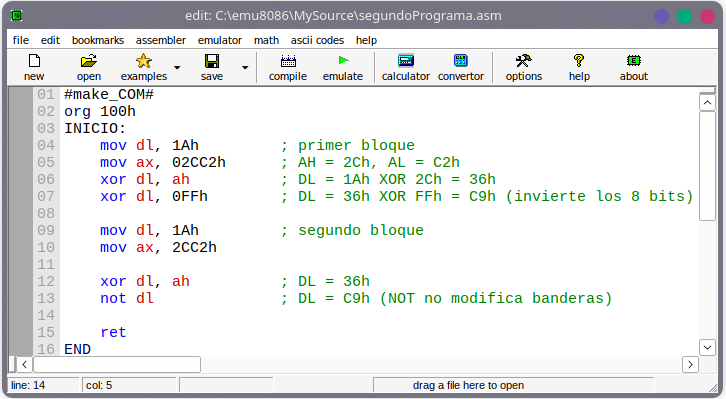
\includegraphics[width=0.85\textwidth]{img/5.png}
    \caption{Código del segundo programa en el editor de EMU8086.}
    \label{fig:bloque1.asm}
\end{figure}

\begin{figure}[H]
    \centering
    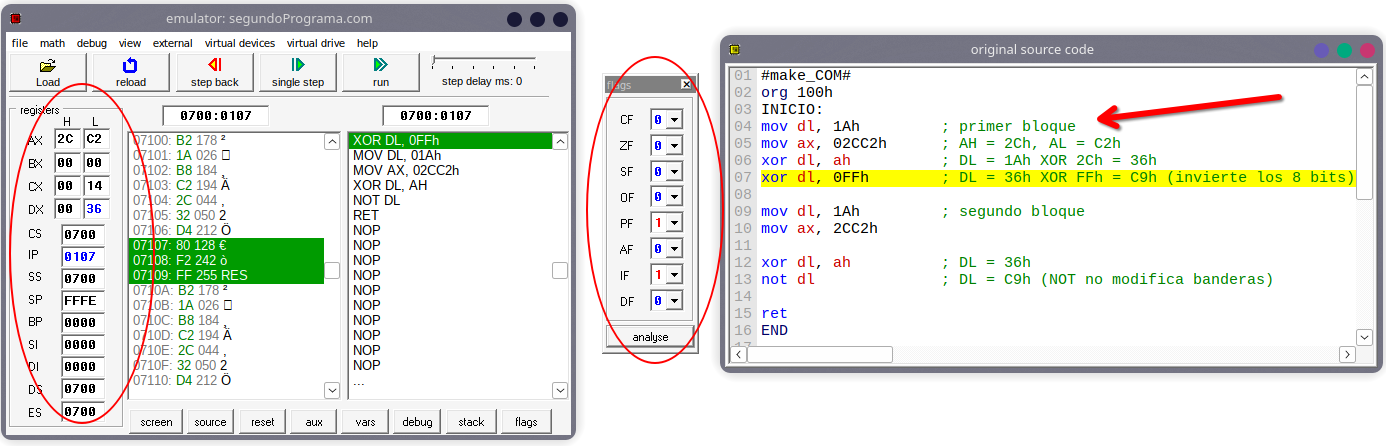
\includegraphics[width=0.85\textwidth]{img/5(1).png}
    \caption{Registros y estado de flags en la ejecución del primer bloque.}
    \label{fig:bloque1.asm}
\end{figure}

\begin{figure}[H]
    \centering
    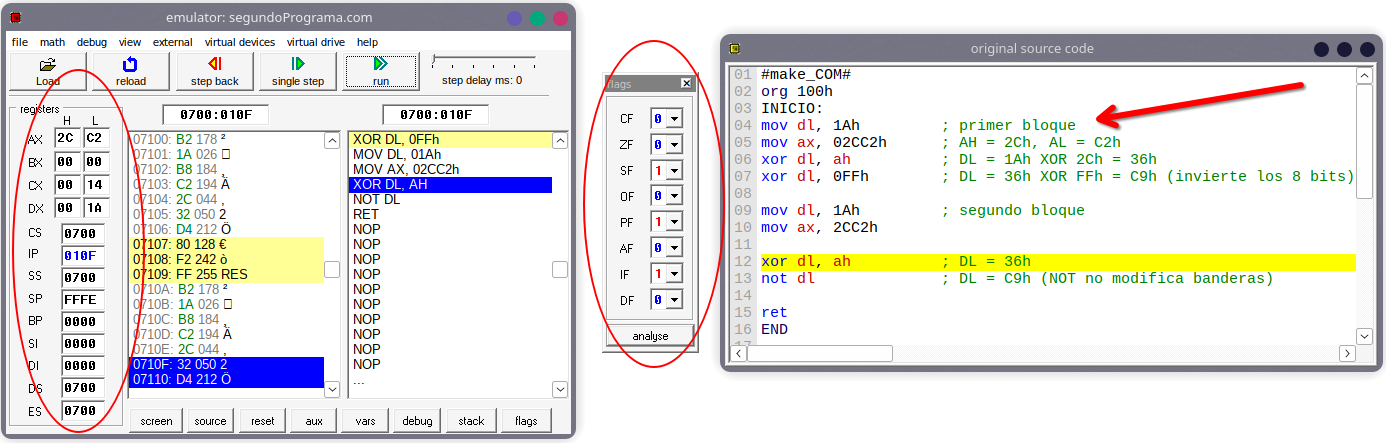
\includegraphics[width=0.85\textwidth]{img/5(2).png}
    \caption{Registros y estado de flags en la ejecución del segundo bloque.}
    \label{fig:bloque2.asm}
\end{figure}
 
\begin{table}[htbp]
  \centering
  \caption{Ejecución paso a paso del segundo programa original.}
  \label{tab:p2-original}
  \begin{tabular}{|l|c|c|c|c|c|c|}
    \hline
    \textbf{Instrucción} & \textbf{Operación} & \textbf{DL} & \textbf{AH} & \textbf{S} & \textbf{Z} & \textbf{P} \\
    \hline
    \multicolumn{7}{|l|}{\textbf{Primer bloque}} \\
    \hline
    \texttt{mov dl, 1Ah} & carga & 1Ah & -- & -- & -- & -- \\
    \hline
    \texttt{mov ax, 02CC2h} & carga & 1Ah & 2Ch & -- & -- & -- \\
    \hline
    \texttt{xor dl, ah} & 1Ah XOR 2Ch & 36h & 2Ch & 0 & 0 & 1 \\
    \hline
    \texttt{xor dl, 0FFh} & 36h XOR FFh & C9h & 2Ch & 1 & 0 & 1 \\
    \hline
    \multicolumn{7}{|l|}{\textbf{Segundo bloque}} \\
    \hline
    \texttt{mov dl, 1Ah} & carga & 1Ah & 2Ch & -- & -- & -- \\
    \hline
    \texttt{mov ax, 2CC2h} & carga & 1Ah & 2Ch & -- & -- & -- \\
    \hline
    \texttt{xor dl, ah} & 1Ah XOR 2Ch & 36h & 2Ch & 0 & 0 & 1 \\
    \hline
    \texttt{not dl} & NOT 36h & C9h & 2Ch & 0 & 0 & 1 \\
    \hline
  \end{tabular}
 
  \smallskip
  {\small (--) La instrucción no modifica esa bandera. \texttt{NOT} tampoco modifica ninguna bandera.}
\end{table}
 
\textbf{Observaciones.} En ambos bloques DL termina en C9h, pero la bandera S queda en 1 en el primero y en 0 en el segundo: \texttt{XOR dl, 0FFh} es una operación lógica y actualiza las banderas con su resultado, mientras que \texttt{NOT dl} solo invierte los bits y conserva las banderas de la instrucción anterior.
 
\subsubsection{Variante con \texttt{xor ah, dl}}
 
Se modificó la tercera y la séptima instrucción del programa, sustituyendo \texttt{xor dl, ah} por \texttt{xor ah, dl}:

\begin{figure}[H]
    \centering
    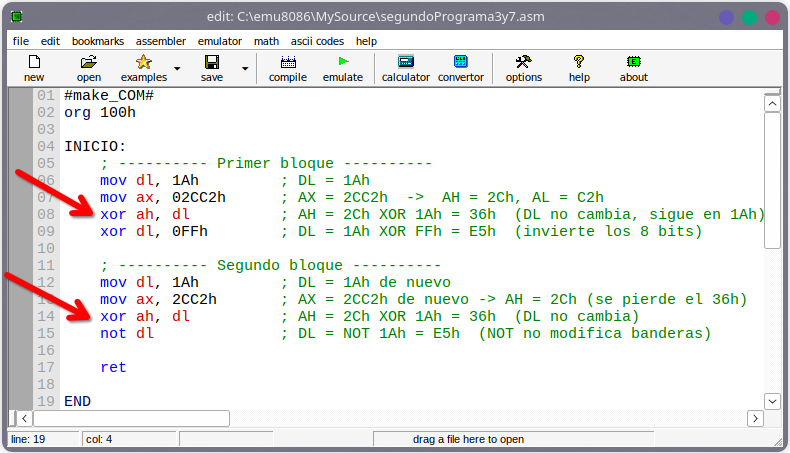
\includegraphics[width=0.91\textwidth]{img/7.png}
    \caption{Bloques del segundo programa con \texttt{xor ah, dl}.}
    \label{fig:segundoPrograma3y7.asm}
\end{figure}

\begin{figure}[H]
    \centering
    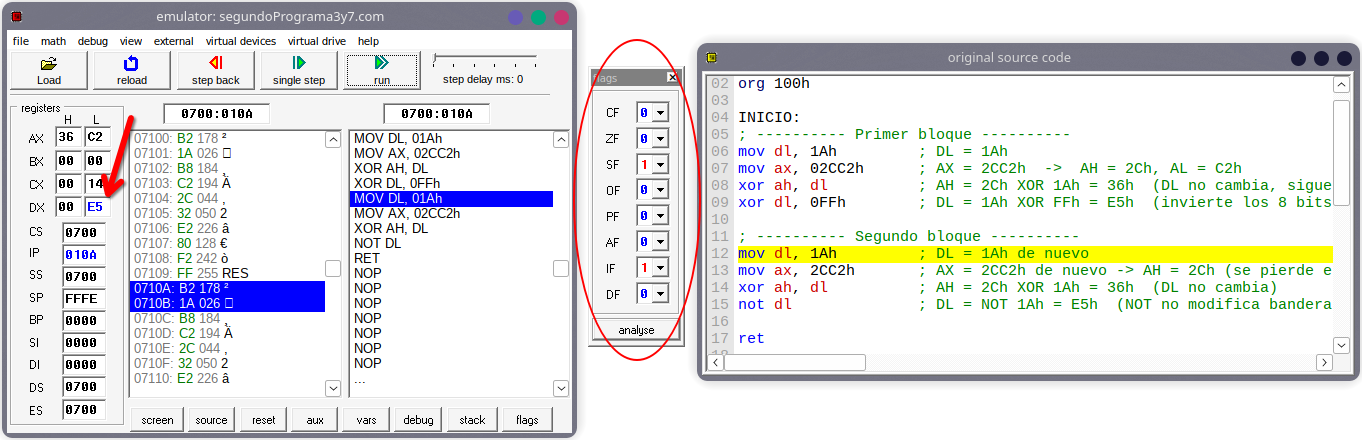
\includegraphics[width=0.91\textwidth]{img/7(1).png}
    \caption{Estado de DL y de las banderas al final del primer bloque.}
    \label{fig:segundoPrograma3y7.asm}
\end{figure}

\begin{figure}[H]
    \centering
    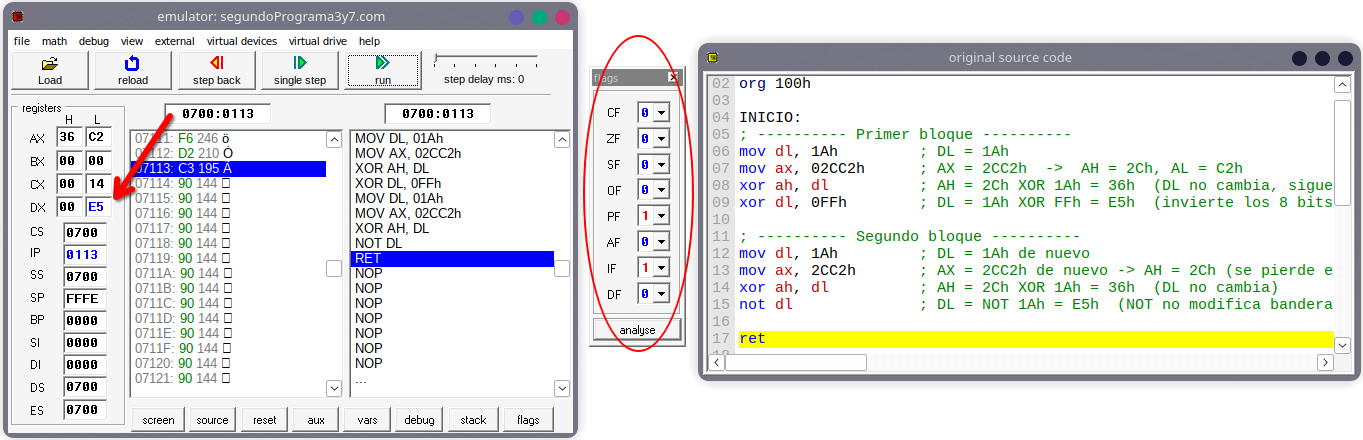
\includegraphics[width=0.91\textwidth]{img/7(2).png}
    \caption{Estado de DL y de las banderas al final del segundo bloque}
    \label{fig:segundoPrograma3y7.asm}
\end{figure}{Estado de DL y de las banderas al final del segundo bloque}
 
\begin{table}[htbp]
  \centering
  \caption{Ejecución del segundo programa con \texttt{xor ah, dl}.}
  \label{tab:p2-variante}
  \begin{tabular}{|l|c|c|c|c|c|c|}
    \hline
    \textbf{Instrucción} & \textbf{Operación} & \textbf{DL} & \textbf{AH} & \textbf{S} & \textbf{Z} & \textbf{P} \\
    \hline
    \multicolumn{7}{|l|}{\textbf{Primer bloque}} \\
    \hline
    \texttt{xor ah, dl} & 2Ch XOR 1Ah & 1Ah & 36h & 0 & 0 & 1 \\
    \hline
    \texttt{xor dl, 0FFh} & 1Ah XOR FFh & E5h & 36h & 1 & 0 & 0 \\
    \hline
    \multicolumn{7}{|l|}{\textbf{Segundo bloque}} \\
    \hline
    \texttt{xor ah, dl} & 2Ch XOR 1Ah & 1Ah & 36h & 0 & 0 & 1 \\
    \hline
    \texttt{not dl} & NOT 1Ah & E5h & 36h & 0 & 0 & 1 \\
    \hline
  \end{tabular}
\end{table}
  
\textbf{Observaciones.} Ahora el resultado de la primera operación se guarda en AH (36h) y DL conserva su valor inicial (1Ah). Al final DL vale E5h en lugar de C9h, AH vale 36h en lugar de 2Ch, y en el primer bloque la bandera P pasa de 1 a 0 (E5h tiene cinco unos).
 
\subsubsection{Control directo de banderas}
 
Se insertaron instrucciones que modifican banderas sin depender del resultado de ninguna operación (se tomó como base el programa original):
 
\begin{figure}[H]
    \centering
    \includegraphics[width=0.91\textwidth]{img/8.png}
    \caption{Bloques del segundo programa con instrucciones de control de banderas.}
    \label{fig:controlBanderas.asm}
\end{figure}
 
\begin{table}[htbp]
  \centering
  \caption{Efecto de las instrucciones de control de banderas.}
  \label{tab:p2-banderas}
  \begin{tabular}{|l|p{1.9cm}|p{2.6cm}|p{3.8cm}|}
    \hline
    \textbf{Instrucción} & \textbf{Bandera} & \textbf{Valor} & \textbf{Observación} \\
    \hline
    \texttt{stc} & C & 1 & Activa C sin importar ningún resultado. \\
    \hline
    \texttt{std} & D & 1 & Activa la bandera de dirección. \\
    \hline
    \texttt{cli} & I & 0 & Desactiva las interrupciones. \\
    \hline
    \texttt{clc} & C & 0 & Desactiva C. \\
    \hline
    \texttt{cld} & D & 0 & Desactiva la bandera de dirección. \\
    \hline
    \texttt{sti} & I & 1 & Activa las interrupciones. \\
    \hline
    \texttt{xor dl, ah} & S, Z, P, C, O & S=0, Z=0, P=1, C=O=0 & Se actualizan según el resultado; D e I no cambian. \\
    \hline
  \end{tabular}
\end{table}
 
\begin{figure}[H]
    \centering
    \includegraphics[width=0.91\textwidth]{img/8(1).png}
    \caption{Emulando las instrucciones, banderas \textit{C, D} e \textit{I} modificadas.}
    \label{fig:controlBanderas.asm}
\end{figure}

\textbf{Conclusión de la actividad.} Existen dos tipos de banderas: las que dependen del resultado de una operación (S, Z, P, y también C y O en las operaciones lógicas) y las que se controlan explícitamente con instrucciones propias (C, D e I). Una operación lógica posterior puede cambiar C (la deja en 0), pero no altera D ni I.
 
% ------------------------------------------------------------
\subsection{Tercer programa: máscaras con AND y TEST}
 
\textbf{Objetivo.} Aprender a comprobar el estado de un bit usando una máscara y comparar \texttt{AND} con \texttt{TEST}: ambas actualizan las banderas igual, pero \texttt{TEST} no guarda el resultado.
 
\begin{figure}[H]
    \centering
    \includegraphics[width=0.86\textwidth]{img/9.png}
    \caption{Código del tercer programa en el editor de EMU8086.}
    \label{fig:tercerPrograma.asm}
\end{figure}

\subsubsection{Máscara 40h (bit D6)}
 
\begin{table}[htbp]
  \centering
  \caption{Ejecución del tercer programa con la máscara 40h.}
  \label{tab:p3-40}
  \begin{tabular}{|l|c|c|c|c|p{4.2cm}|}
    \hline
    \textbf{Instrucción} & \textbf{AH} & \textbf{S} & \textbf{Z} & \textbf{P} & \textbf{Interpretación} \\
    \hline
    \texttt{mov ah, 0B9h} & B9h & -- & -- & -- & \texttt{MOV} no modifica banderas. \\
    \hline
    \texttt{and ah, 40h} & 00h & 0 & 1 & 1 & Z=1: el bit D6 de B9h vale 0. \\
    \hline
    \texttt{or ah, 01h} & 01h & 0 & 0 & 0 & Resultado distinto de cero. \\
    \hline
    \texttt{mov ah, 0B9h} & B9h & 0 & 0 & 0 & Se restaura AH; banderas sin cambio. \\
    \hline
    \texttt{test ah, 40h} & B9h & 0 & 1 & 1 & AH se conserva; Z=1 indica D6=0. \\
    \hline
  \end{tabular}
\end{table}
 
\begin{figure}[H]
    \centering
    \includegraphics[width=0.86\textwidth]{img/9(1).png}
    \caption{Emulador después de la instrucción \textit{AND}.}
    \label{fig:tercerPrograma.asm}
\end{figure}

\begin{figure}[H]
    \centering
    \includegraphics[width=0.86\textwidth]{img/9(2).png}
    \caption{Emulador después de la instrucción \textit{TEST}.}
    \label{fig:p3-test}
\end{figure}

\textbf{Interpretación.} Al ejecutar las dos primeras instrucciones se activaron Z y P, y AH quedó en 00h. El resultado indica que el bit D6 del dato B9h (1011 1001) vale 0. Con \texttt{TEST} las banderas son las mismas, pero AH conserva su valor B9h.
 
\subsubsection{Máscara 08h (bit D3)}
 
Se cambió el dato 40h por 08h en la segunda y quinta instrucción.
 
\begin{figure}[H]
    \centering
    \includegraphics[width=0.86\textwidth]{img/10.png}
    \caption{Emulador con la máscara 08h.}
    \label{fig:tercerPrograma08h.asm}
\end{figure}

\begin{table}[htbp]
  \centering
  \caption{Ejecución del tercer programa con la máscara 08h.}
  \label{tab:p3-08}
  \begin{tabular}{|l|c|c|c|c|p{4.2cm}|}
    \hline
    \textbf{Instrucción} & \textbf{AH} & \textbf{S} & \textbf{Z} & \textbf{P} & \textbf{Interpretación} \\
    \hline
    \texttt{mov ah, 0B9h} & B9h & -- & -- & -- & \texttt{MOV} no modifica banderas. \\
    \hline
    \texttt{and ah, 08h} & 08h & 0 & 0 & 0 & Z=0: el bit D3 de B9h vale 1. \\
    \hline
    \texttt{or ah, 01h} & 09h & 0 & 0 & 1 & Resultado distinto de cero. \\
    \hline
    \texttt{mov ah, 0B9h} & B9h & 0 & 0 & 1 & Se restaura AH; banderas sin cambio. \\
    \hline
    \texttt{test ah, 08h} & B9h & 0 & 0 & 0 & AH se conserva; Z=0 indica D3=1. \\
    \hline
  \end{tabular}
\end{table}
 
\begin{figure}[H]
    \centering
    \includegraphics[width=0.86\textwidth]{img/10(1).png}
    \caption{Emulador con la máscara \textit{08h} después de la instrucción \textit{AND}.}
    \label{fig:tercerPrograma08h.asm}
\end{figure}

\begin{figure}[H]
    \centering
    \includegraphics[width=0.86\textwidth]{img/10(2).png}
    \caption{Emulador con la máscara \textit{08h} después de la instrucción \textit{TEST}.}
    \label{fig:tercerPrograma08h.asm}
\end{figure}

\textbf{Interpretación.} Con la máscara 08h se prueba el bit D3. Como en B9h ese bit vale 1, el resultado de la operación es distinto de cero y la bandera Z queda en 0: el resultado del programa cambió respecto al caso de la máscara 40h.
 
% ============================================================
\section{Análisis de resultados}
 
\begin{enumerate}
  \renewcommand{\labelenumi}{\alph{enumi})}
  \renewcommand{\labelenumii}{\arabic{enumii}.}
 
  \item \textbf{Primer programa.}
  \begin{enumerate}
    \item \textbf{¿Qué objetivos se buscan al usar la máscara1 (F0h) con las tres diferentes instrucciones lógicas?}\\
    Actuar solo sobre el nibble alto (bits D7 a D4) y dejar intacto el bajo. Con \texttt{AND} se conserva el nibble alto y se borra el bajo (9Ah $\rightarrow$ 90h). Con \texttt{OR} se ponen en 1 los bits del nibble alto (9Ah $\rightarrow$ FAh). Con \texttt{XOR} se invierten los bits del nibble alto (9Ah $\rightarrow$ 6Ah). Así, la máscara permite borrar, poner en 1 o invertir un grupo de bits sin afectar a los demás.
 
    % VERIFICAR con las capturas: con los datos de la guía, el resultado de 16 bits del AND es 0C02h (bit 15 = 0).
    \item \textbf{En la primera instrucción AND el bit D7 termina en alto y se activa la bandera S; en la segunda también termina en alto, pero no se activa la bandera, ¿por qué?}\\
    Porque la bandera S copia el bit más significativo \emph{del tamaño de la operación}: el bit 7 en las operaciones de 8 bits y el bit 15 en las de 16 bits. La primera instrucción opera con registros de 8 bits (DL) y su bit 7 vale 1, por lo que S se activa. La segunda opera con registros de 16 bits (CX) y su bit 15 vale 0, por lo que S no se activa, aunque el bit 7 del resultado pueda valer 1 (por ejemplo, con \texttt{OR} el resultado 2FCFh tiene D7 = 1 y D15 = 0).
 
    \item \textbf{Cuando se ejecuta la tercera instrucción lógica, con AND u OR las banderas reaccionan de forma similar, pero con XOR no, ¿por qué?}\\
    Porque \texttt{and cx, cx} y \texttt{or cx, cx} devuelven el mismo valor de CX (A AND A = A y A OR A = A), de modo que las banderas quedan igual que tras la operación anterior. En cambio \texttt{xor cx, cx} da siempre 0 (A XOR A = 0): CX se borra y se activa Z.
 
    \item \textbf{En el programa se declaran datos para hacer las operaciones, ¿dónde se guardan estos datos?}\\
    En la memoria, dentro del mismo segmento del programa (en un archivo \texttt{.COM}, CS = DS), a continuación de la última instrucción. Las instrucciones \texttt{mov} los leen con direccionamiento directo.
  \end{enumerate}
 
  \item \textbf{Segundo programa.}
  \begin{enumerate}
    \item \textbf{El resultado del primer y del segundo bloque es idéntico en DL, pero el estado de las banderas no lo es, ¿por qué?}\\
    Porque \texttt{xor dl, 0FFh} es una operación lógica que actualiza las banderas según su resultado (C9h: S=1, Z=0, P=1), mientras que \texttt{not dl} solo invierte los bits y no modifica ninguna bandera. En el segundo bloque las banderas quedan como las dejó \texttt{xor dl, ah} (resultado 36h: S=0, Z=0, P=1).
 
    \item \textbf{Al modificar el programa, tanto los resultados como las banderas terminaron en distintos estados, ¿cuáles fueron los cambios específicos que observó?}\\
    Con \texttt{xor ah, dl} el resultado se guarda en AH (36h) y DL conserva 1Ah. Después, \texttt{xor dl, 0FFh} y \texttt{not dl} dejan DL en E5h en lugar de C9h. En el primer bloque la bandera P pasó de 1 a 0 (E5h tiene cinco unos) y S sigue en 1. En el segundo bloque las banderas quedan en S=0, Z=0, P=1.
  \end{enumerate}
 
  \item \textbf{Tercer programa.}
  \begin{enumerate}
    \item \textbf{¿Cuál es la diferencia fundamental entre las instrucciones AND y TEST?}\\
    Ambas realizan la operación AND bit a bit y actualizan las banderas de la misma forma, pero \texttt{AND} guarda el resultado en el operando destino (modificándolo), mientras que \texttt{TEST} descarta el resultado y deja intacto el dato. Por eso, tras \texttt{test ah, 40h}, AH conserva el valor B9h.
 
    \item \textbf{¿Qué relación existe entre los bits que deseamos probar y el valor específico de la máscara seleccionada?}\\
    La máscara debe tener 1 en las posiciones de los bits que se quieren probar y 0 en las demás. Si tras el \texttt{AND} o \texttt{TEST} Z=1, todos los bits probados valen 0; si Z=0, al menos uno vale 1. Por ejemplo, 40h (0100 0000) prueba el bit D6 y 08h (0000 1000) prueba el bit D3.
  \end{enumerate}
\end{enumerate}
 
% ============================================================
\section{Tarea complementaria}
 
\subsection{Almacenamiento de los datos declarados}
 
Los datos que declara el programa se almacenan en la memoria, dentro del mismo segmento donde está el código (en un \texttt{.COM}, CS = DS), a continuación de la última instrucción (después de \texttt{ret}). El ensamblador asigna a cada etiqueta (\texttt{dato1}, \texttt{dato2}, \ldots) el desplazamiento que le corresponde.
 
\subsection{Directivas DB y DW}
 
\begin{itemize}
  \item \texttt{DB} (\textit{Define Byte}): reserva 1 byte (8 bits) por cada valor y lo inicializa. Ejemplo: \texttt{dato1 db 9Ah}.
  \item \texttt{DW} (\textit{Define Word}): reserva 2 bytes (16 bits) por cada valor. En memoria se guarda primero el byte menos significativo (\textit{little endian}): \texttt{dato2 dw 02CC2h} queda como C2h seguido de 2Ch.
  \item No son instrucciones del procesador sino directivas del ensamblador: no se ejecutan, solo indican cómo organizar los datos en memoria.
\end{itemize}
 
\subsection{Programa de manipulación de bits}
 
\textbf{Enunciado.} Dado un dato almacenado en AX, invertir los bits impares desde D5 hasta D1, borrar los bits pares desde D6 hasta D2 y poner en 1 los bits D7 y D0.
 
\textbf{Solución.} Se trabaja sobre AL (bits D7 a D0) con tres máscaras:
\begin{itemize}
  \item \texttt{XOR} con 0010\,1010b (2Ah): invierte D5, D3 y D1.
  \item \texttt{AND} con 1010\,1011b (ABh): borra D6, D4 y D2 y conserva los demás.
  \item \texttt{OR} con 1000\,0001b (81h): pone en 1 D7 y D0.
\end{itemize}
 
\begin{lstlisting}[style=asm]
#make_COM#
org 100h
INICIO:
    mov ax, dato        ; AX = dato (se procesa AL, bits D7..D0)
    xor al, 00101010b   ; invierte D5, D3 y D1
    and al, 10101011b   ; borra D6, D4 y D2
    or  al, 10000001b   ; pone en 1 D7 y D0
    ret
 
dato dw 006Dh           ; dato de prueba: AL = 6Dh = 0110 1101b
END
\end{lstlisting}
 
\figuraimagen{tarea-codigo.png}{Código del programa de manipulación de bits.}{fig:tarea-codigo}{código fuente de la tarea complementaria}
 
\begin{table}[htbp]
  \centering
  \caption{Seguimiento del programa con el dato de prueba 6Dh.}
  \label{tab:tarea}
  \begin{tabular}{|l|c|c|}
    \hline
    \textbf{Instrucción} & \textbf{AL (hex)} & \textbf{AL (binario)} \\
    \hline
    \texttt{mov ax, dato} & 6Dh & 0110 1101 \\
    \hline
    \texttt{xor al, 00101010b} & 47h & 0100 0111 \\
    \hline
    \texttt{and al, 10101011b} & 03h & 0000 0011 \\
    \hline
    \texttt{or al, 10000001b} & 83h & 1000 0011 \\
    \hline
  \end{tabular}
\end{table}
 
\figuraimagen{tarea-resultado.png}{Registros del emulador al finalizar el programa de manipulación de bits.}{fig:tarea-resultado}{emulador con AX = 0083h al final del programa}
 
El resultado final cumple el enunciado: D7 y D0 valen 1, D6, D4 y D2 valen 0, y D5, D3 y D1 quedaron invertidos respecto al dato original.
 
% ============================================================
\section{Conclusiones}
 
\begin{itemize}
  \item Las instrucciones lógicas operan bit a bit, y combinadas con una máscara permiten borrar (\texttt{AND}), poner en 1 (\texttt{OR}) o invertir (\texttt{XOR}) bits específicos de un dato sin afectar a los demás.
  \item El registro de banderas refleja el resultado de la última operación que lo modifica: Z indica resultado cero, S copia el bit más significativo del tamaño de la operación y P indica un número par de unos en el byte bajo. \texttt{AND}, \texttt{OR} y \texttt{XOR} dejan siempre C y O en 0.
  \item \texttt{XOR} de un registro consigo mismo lo pone a cero y activa Z, mientras que \texttt{AND} y \texttt{OR} de un registro consigo mismo no cambian su valor.
  \item \texttt{XOR} con FFh y \texttt{NOT} producen el mismo resultado, pero solo \texttt{XOR} actualiza las banderas; \texttt{NOT} no modifica ninguna.
  \item Algunas banderas (C, D e I) se pueden activar o desactivar directamente con instrucciones específicas (\texttt{STC/CLC}, \texttt{STD/CLD}, \texttt{STI/CLI}), independientemente del resultado de una operación.
  \item \texttt{TEST} permite probar bits con una máscara sin destruir el dato, a diferencia de \texttt{AND}. La máscara debe tener 1 en los bits que se desean probar.
  \item Las directivas \texttt{DB} y \texttt{DW} permiten declarar datos de 8 y 16 bits que quedan almacenados en memoria junto al programa, y que el procesador guarda en formato \textit{little endian}.
\end{itemize}

\end{document}